\chapter{Signals processing and classification of data force}
\label{ch:forceData}

\section{Introduction and chapter's structure}
In the previous chapter, we analysed and extracted features of force data and inertial sensors data of the patients from the same experiment . Thus, once we compared both systems and determined the relationship between them, we proceed to conclude whether we can classify force data from patients and control subjects.

Along this chapter, we are going to explain Hardware used in this experiment, the procedure to gathering the data, the process carried out to calculate the relevant signals, different techniques to feature extraction as well as the results obtained after the classification of this information.

\section{PLS}
Partial least squares regression (PLS regression) is a statistical method that bears some relation to principal components regression; instead of finding hyperplanes of minimum variance between the response and independent variables, it finds a linear regression model by projecting the predicted variables and the observable variables to a new space \cite{pls_pca} 
%\cite{pls_wiki}.

This algorithm is based on linear transition from a large number of original descriptors to a new variable space based on small number of orthogonal factors (latent variables), i.e factors are mutually independent (orthogonal) linear combinations of original descriptors\cite{pls_pca} .
%\cite{pls}.

We used in the last chapter PCA algorithm to extract features of the gait data. This new method is very similar but there are clear differences. Both PCA and PLS are used as a dimension reduction methodology. However, PCA is applied without the consideration of the correlation between the dependent variable and the independent variables, while PLS is applied based on the correlation. Therefore, we call PCA as an unsupervised dimension reduction methodology, and call PLS as a supervised dimension reduction methodology, i.e it has a phase of training and another of evaluation or testing\cite{pls_pca}.

Once establish the most important differences between them, we are going to explain the fundamentals of this algorithm. 
Assume X is a \textit{n×p} matrix and Y is a \textit{n×q} matrix. The PLS technique works by successively extracting factors from both X and Y such that covariance between the extracted factors is maximized. In our particular case, we will assume that we have a single response variable i.e., Y is \textit{n×1} and X is \textit{n×p}, as before.

\begin{center}
	$ Y= UQ’+F $

$ X=TP’+E $
\end{center}

where Q\textit{(qxr)} and P \textit{(pxr)} are the matrices of coefficients (orthogonal loading matrices) , F \textit{(nxq)} and E \textit{(nxp)} are the error term and, U \textit{(nxr)} and T \textit{(nxr)} matrices that are, respectively, projections of X and projections of Y.

Decomposition is finalized so as to maximize covariance between T and U. All algorithms to solve this follow an iterative process to extract the T(X-scores) and U(Y-scores)\cite{pls_pca}. 

The factors or scores for X and Y are extracted successively and the number of factors extracted \textit{(r)} depends on the rank of X and Y. In our case, Y is a vector and all possible X factors will be extracted.
Each extracted X-score are linear combinations of X. Thus, the score T of X is of the form: 

\begin{center}
	$ T= XW $
\end{center}

Where  W is a matriz obtained as follow:

\begin{center}
	$ W= conv(X,Y); $
$ W = W/||W|| $
\end{center}

With r (latents variables) columns.

\section{Signals processing and feature extraction}
The database used in this experiment  is different in contrast with the above case. This contains measure of gait from 27 patients (mean age: 66.3 years; 63 \% men) and 18 healthy controls (mean age: 66.3 years; 63\% men). The database includes the vertical ground reaction force records of subjects as they walked at their usual. They wear underneath each foot 8 sensors\cite{Instr6} that measure force as a function time. The output of each of these 16 sensors has been digitized and recorded at 100 samples per second.

Once data have been gathered while subjects were walking during two minutes approximately, we read this information from the text file. This file contains the force of each sensors as well as the sum of force of the right and left feet.

With these values, we can obtain the center of pressure Antero-Posterior and Medio-Lateral  as indicate the equation \ref*{COP}. To do this, we have to define the position of the sensors. When a person is comfortably standing with both legs parallel to each other, sensor locations inside the insole can be described (according to \cite{Instr6}) as lying approximately at the following (X,Y) coordinates, assuming that the origin (0,0) is just between the legs and the person is facing towards the positive side of the Y axis:
\begin{figure}[H]
	\centering
	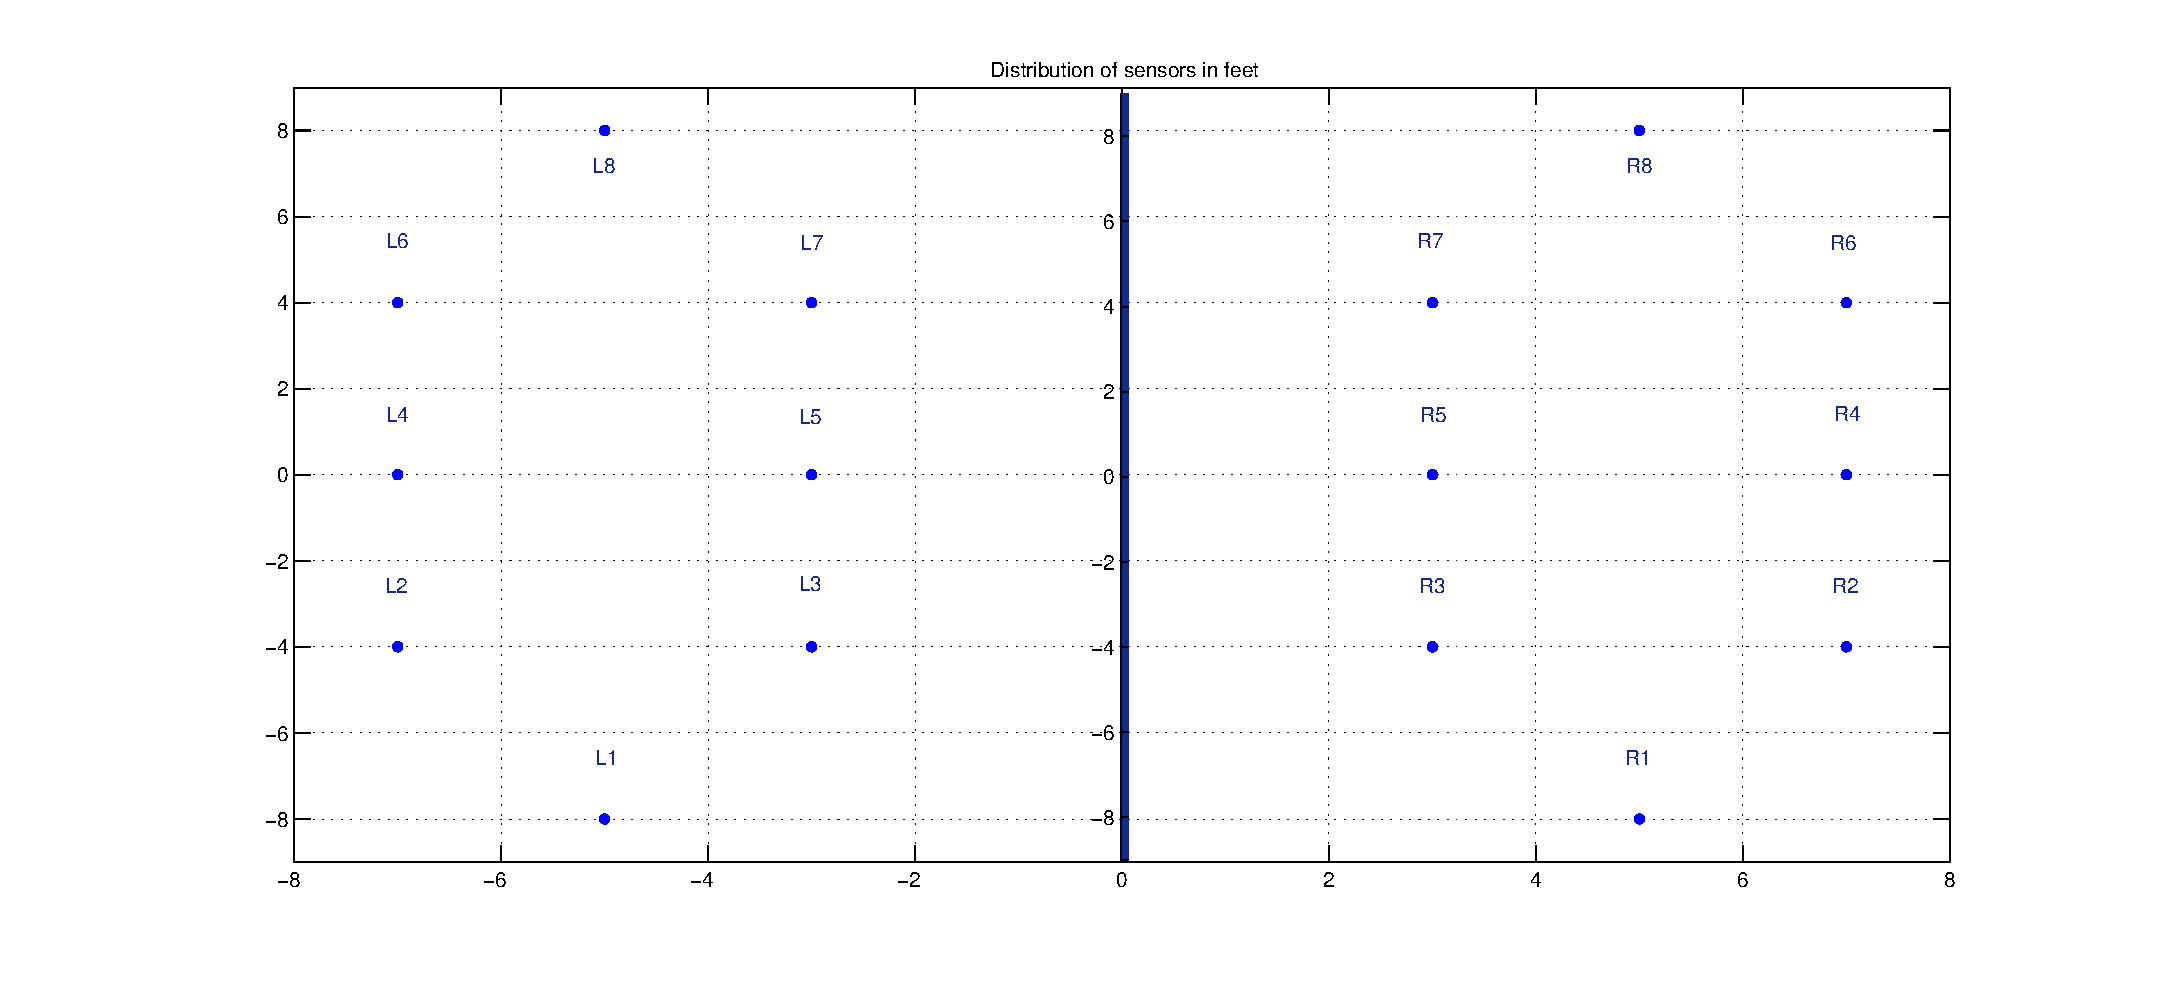
\epsfig{file=figures/forceData/DistributionSensors, width=18cm}
	\caption{Distribution of the sensors underneath both feet.}
	\label{fig:DistributionSensors}
\end{figure}

The X and Y numbers are in an arbitrary coordinate system reflecting the relative (arbitrarily scaled) positions of the sensors within each insole. During walking, the sensors inside each insole remain at the same relative position, but the two feet are no longer parallel to each other. Thus, this coordinate system enables a calculation of a proxy for the location of the center of pressure (COP) under each foot.

Hereafter, we separate the differents steps because the subjects carry out several steps during the experiment. We detect this when the COP signal has a strong fall in one of the feet. One we have delimited the intervals of the signals, we figure out the average of them using cross correlation to synchronise the cycles properly. We can see the result in the following figure:
\begin{figure}[H]
	\centering
	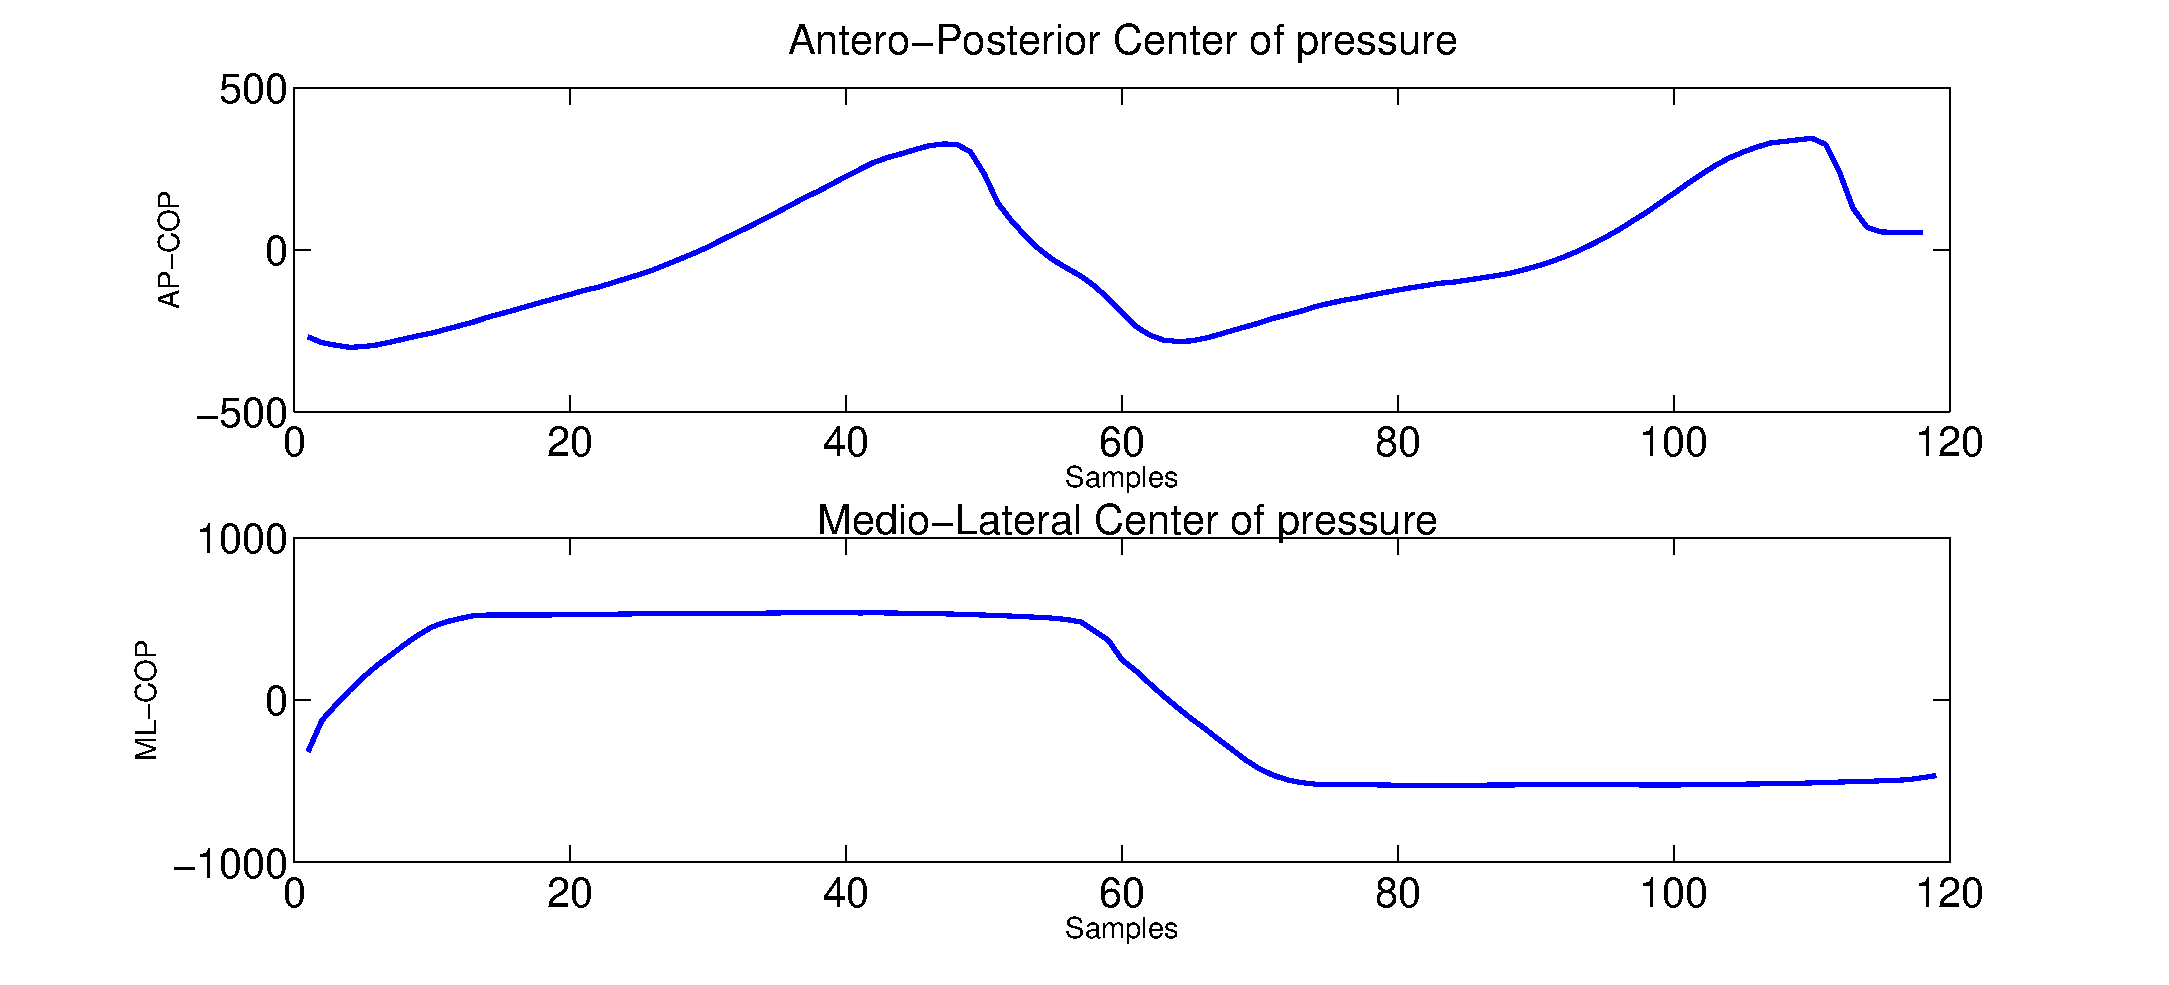
\epsfig{file=figures/forceData/COP, width=18cm}
	\caption{Center of pressure in AP and ML direction.}
	\label{fig:COP}
\end{figure}

Thus, after this, we only have two signals ML and AP COP that represent one step of the patient. It is not absolutely necessary but it allows us to obtain a average of each repeat, being this more appropriate to characterise the subjects.

We use these signals to apply PCA as in the previous experiment. We match ML-COP and AP COP in the same column corresponding to the same subject and rearrange both patients and healthy controls in the same data matrix to apply this algorithm.

As we explained before, PCA is an unsupervised method, so we will use PLS algorithm to extract the relevant information and carry out a better classification of the data. We calculated X-score of the all data for different numbers of components (latent variables). The results after the classification can be seen in the next section.


\section{Classification and Results discurssion}